\documentclass[zihao=-4]{ctexart}
\usepackage[normalem]{ulem}
\useunder{\uline}{\ul}{}
%********************导言区宏包引入********************
\usepackage{xeCJK}
\usepackage{amssymb}
\usepackage{amsmath}
\usepackage{listings} %代码
\usepackage{graphicx}
\usepackage{multicol} %回车换段
\usepackage{xcolor}
\usepackage{geometry} %页面设置
\usepackage{fontspec}
\usepackage{setspace}
\usepackage{times}
\usepackage{fancyhdr} %页眉页脚
\pagestyle{fancy}
\usepackage{float} %表格位置
\usepackage{titlesec} %设置
\usepackage{titletoc}
\usepackage{ctex}
\usepackage{gbt7714}    %控制参考文献格式为国标
\usepackage{multirow}
\usepackage{booktabs}   %表格相关
\usepackage{setspace}   %设置行距
\usepackage{caption} %caption
\usepackage{subcaption} %子图的caption
\usepackage{changepage} %左右缩进


\graphicspath{ {include_picture/} }
\let\algorithm\relax
\let\endalgorithm\relax
\usepackage[ruled,vlined]{algorithm2e}%[ruled,vlined]{
\usepackage{algpseudocode}
\renewcommand{\algorithmicrequire}{\textbf{Input:}} 
\renewcommand{\algorithmicensure}{\textbf{Output:}}
%\renewcommand\thepage{\zihao{-5} ~\arabic{page}~}%页码字号

%定义两个arg
\DeclareMathOperator*{\argmax}{arg\,max}
\DeclareMathOperator*{\argmin}{arg\,min}
\DeclareCaptionLabelSeparator{mysep}{\space\space}  %自定义caption格式
\captionsetup[figure]{labelfont=bf, labelsep=mysep, textfont=bf}   %图片caption格式
\captionsetup[table]{labelfont=bf, labelsep=mysep, textfont={bf}}   %表格caption格式
\bibliographystyle{gbt7714-numerical} %修改了title斜体内容

%********************导言区宏包引入********************
%********************第三方字体引入********************
%\setCJKmainfont[Path=fonts/,BoldFont=simhei.ttf,ItalicFont=simkai.ttf,SlantedFont=simfang.ttf]{simsun.ttc}
%中文字体涵盖黑体、宋体、楷体、仿宋
\setmainfont[Path=fonts/, 
BoldFont = times-new-roman-bold.ttf,
ItalicFont = times-new-roman-italic.ttf,
BoldItalicFont = times-new-roman-bold-italic.ttf
]{times-new-roman.ttf}
\setmonofont[Path=fonts/]{Courier New.ttf}
\setCJKfamilyfont{hwzs}[Path=fonts/]{STKzhongsong.ttf}%使用STZhogsong华文中宋字体
\newcommand{\zhongsong}{\CJKfamily{hwzs}}

%********************第三方字体引入********************


%********************中文字号设置********************
%\newcommand{\chuhao}{\fontsize{42pt}{\baselineskip}\selectfont}
\newcommand{\chuhao}{\fontsize{42pt}{0}}
\newcommand{\xiaochu}{\fontsize{36pt}{0}}
\newcommand{\yihao}{\fontsize{28pt}{0}}
\newcommand{\erhao}{\fontsize{21pt}{0}}
\newcommand{\xiaoer}{\fontsize{18pt}{0}}
\newcommand{\sanhao}{\fontsize{16pt}{0}}
\newcommand{\sihao}{\fontsize{14pt}{0}}
\newcommand{\xiaosi}{\fontsize{12pt}{0}}
\newcommand{\wuhao}{\fontsize{10.5pt}{0}}
\newcommand{\xiaowu}{\fontsize{9pt}{0}}
\newcommand{\liuhao}{\fontsize{8pt}{0}}
\newcommand{\qihao}{\fontsize{5.25pt}{0}}
%********************中文字号设置********************


%********************页边距设置********************
\geometry{left=3cm,right=3.5cm,top=2.5cm,bottom=2.5cm}
%页边距
%********************页边距设置********************
%********************

\begin{document}

%********************页眉页脚设置********************
\lhead{}%设置左页眉为空
\rhead{}%设置左页眉为空
%********************页眉页脚设置********************


%********************标题格式设置********************

%\setcounter{secnumdepth}{0}%该命令取消了章标题前数字label

\CTEXsetup[name={,、},number={\chinese{section}}]{section}
\CTEXsetup[name={(,)},number={\chinese{subsection}}]{subsection}
\CTEXsetup[name={,、},number={\arabic{subsubsection}}]{subsubsection}% 不加会导致目录格式错误
% 设置subsubsection等格式
\titleformat{\section}[block]{\sanhao\bfseries\centering}{\chinese{section}、}{0pt}{}[]
\titleformat{\subsection}[block]{\sihao\bfseries}{(\chinese{subsection})}{0pt}{}[]
\titleformat{\subsubsection}[block]{\xiaosi\bfseries}{\arabic{subsubsection}、}{0pt}{}[]
\titlespacing{\section}{0pt}{25pt}{12pt}
\titlespacing{\subsection}{0pt}{7pt}{7pt}
\titlespacing{\subsubsection}{0pt}{5pt}{4pt}

\titlecontents{section}[1.6em]{\addvspace{2pt}\filright}
{\contentspush{\thecontentslabel\hspace{0.8em}}}
{}{\titlerule*[8pt]{.}\contentspage}

\titlecontents{subsection}[3.2em]{\addvspace{2pt}\filright}
{\contentspush{\thecontentslabel\hspace{0.8em}}}
{}{\titlerule*[8pt]{.}\contentspage}

\titlecontents{subsubsection}[6.4em]{\addvspace{2pt}\filright}
{\contentspush{\thecontentslabel\hspace{0.8em}}}
{}{\titlerule*[8pt]{.}\contentspage}
%********************标题格式设置********************

%\setcounter{section}{-3}  %标题计数器
%\stepcounter{section}

%*******************行间距段前段后*******************
\linespread{1.8}
%行间距为实际行间距乘以1.2,如此处实际为1.5倍行距
\setlength{\parskip}{0.5\baselineskip}
%*******************行间距段前段后*******************



%********************封面部分********************

\includegraphics[scale=1]{include_picture/xiaohui.png}
%格式控制部分
\par \  
\par \ 
\par \ 
\begin{center}

\includegraphics[scale=1]{include_picture/xiaoming.png}
\end{center}
%格式控制部分

\begin{spacing}{3}
    \erhao
    \begin{center}
        \zhongsong\erhao{第三十二届“冯如杯”竞赛主赛道项目论文} %黑体这样调用,其余字体同理
        
        \zhongsong{“冯如杯”竞赛主赛道项目是什么}
    \end{center}
\end{spacing}
%格式控制部分
% \par \ 
% \par \
\par \ 
\par \
\par \ 
\par \
% \begin{center}
%     \sihao
%     \textbf{学院:计算机学院}
%     \par \ 
%     \textbf{本模板原作者:Someday}
% \end{center}

%格式控制部分
\par \ 
\begin{center}
\sanhao
\centerline{\heiti{}}%封面年月去掉
\end{center}

\pagenumbering{gobble} %封面无页码
%\thispagestyle{empty}


\renewcommand{\headrulewidth}{0pt}%没有页眉装饰线
\clearpage
\pagenumbering{roman} %摘要目录页小写罗马

\xiaosi
\section*{摘要}
\begin{spacing}{1.5}
孔子在不经意间这样说过,知之者不如好之者,好之者不如乐之者。我希望诸位也能好好地体会这句话。 “冯如杯”竞赛主赛道项目是什么,发生了会如何,不发生又会如何。 而这些并不是完全重要,更加重要的问题是, 就我个人来说,“冯如杯”竞赛主赛道项目是什么对我的意义,不能不说非常重大。 既然如此, 现在,解决“冯如杯”竞赛主赛道项目是什么的问题,是非常非常重要的。 所以, 问题的关键究竟为何? “冯如杯”竞赛主赛道项目是什么,到底应该如何实现。 现在,解决“冯如杯”竞赛主赛道项目是什么的问题,是非常非常重要的。 所以, 可是,即使是这样,“冯如杯”竞赛主赛道项目是什么的出现仍然代表了一定的意义。 培根在不经意间这样说过,深窥自己的心,而后发觉一切的奇迹在你自己。我希望诸位也能好好地体会这句话。 我认为, 本人也是经过了深思熟虑,在每个日日夜夜思考这个问题。
\end{spacing}
    
\textbf{关键字:}人生,哲学,意义,价值,生命

\newpage
\section*{Abstract}
\begin{spacing}{1.5}
\begin{adjustwidth}{0.42cm}{0.42cm}
\quad
Confucius said in an offhand way that those who know are better than those who are good, and those who are good are better than those who are happy. I hope that you will also appreciate this saying. What is the main track of the "Fengru Cup" competition, what will happen if it happens, and what will happen if it does not. The more important issue is that, personally, what is the main track of the "Fengru Cup" competition means a lot to me. That being the case, it is very, very important for me to solve the question of what is the main track of the Fengru Cup. So, what is the key to the question? What is the main track of the "Fengru Cup" competition and how should it be realized? Now, it is very important to solve the question of what is the main track of the Fengru Cup. So, even so, the emergence of the main track of the "Fengru Cup" competition is still of some significance. Bacon said, "Look deep into your own heart and realize that the miracle is in you. I hope you all can also appreciate this statement. I think that I, too, have thought deeply about this question every day and night.\par
\textbf{Keywords: Life, philosophy, meaning, value, life}
\end{adjustwidth}
\end{spacing}



%********************摘要部分********************


%********************目录部分********************
\clearpage
\tableofcontents
\clearpage
%********************目录部分********************



\renewcommand{\headrulewidth}{0.4pt} %恢复页眉装饰线

%********************正文页眉部分********************
%\lhead{} 
\chead{\xiaowu 北京航空航天大学第三十二届“冯如杯”竞赛主赛道参赛作品} %设置居中页眉
%********************正文页眉部分********************

\pagenumbering{arabic} %正文页码从1开始,用阿拉伯数字
\setcounter{page}{1} 

\section{简介}
\begin{spacing}{1.5}
叔本华曾经提到过,意志是一个强壮的盲人,倚靠在明眼的跛子肩上。我希望诸位也能好好地体会这句话。 我们都知道,只要有意义,那么就必须慎重考虑。 可是,即使是这样,“冯如杯”竞赛主赛道项目是什么的出现仍然代表了一定的意义。 我们都知道,只要有意义,那么就必须慎重考虑。 现在,解决“冯如杯”竞赛主赛道项目是什么的问题,是非常非常重要的。 所以, 要想清楚,“冯如杯”竞赛主赛道项目是什么,到底是一种怎么样的存在。 对我个人而言,“冯如杯”竞赛主赛道项目是什么不仅仅是一个重大的事件,还可能会改变我的人生。\par

% 段落间可加入\par进行换行,代替两行回车的写法

本文的主要贡献如下:\par
\begin{itemize}
	\item 莎士比亚在不经意间这样说过,抛弃时间的人,时间也抛弃他
	\item 易卜生曾经提到过,伟大的事业,需要决心,能力,组织和责任感
	\item 文森特·皮尔在不经意间这样说过,改变你的想法,你就改变了自己的世界
\end{itemize}
	
\section{相关工作}
可加入背景、相关工作的介绍

\subsection{二级标题格式}
\subsubsection{三级标题格式}
未进行subsubsubsection四级及以上标题格式的设置\par

此处是关于引用的参考~\cite{Squeez},可从Google Scholar、DBLP等网站获取bibtex源格式~\cite{Goodfellow_2015},粘贴至references.bib文件\cite{Xu_2017Squueze}中,之后在此处使用cite调用对应名称即可~\cite{Carlini_2016}\par

\section{理论与算法}

此处插入一些公式
\begin{align}
\underset{{\bf I}_c \sim \boldsymbol\Im_c}{\mathrm{\text P}} \Big( \mathcal C({\bf I}_c) \neq \mathcal C({\bf I}_c + \boldsymbol \rho) \Big) \geq \delta ~~~\text{s.t.}~~||\boldsymbol\rho||_p \leq \xi,
\label{eq:def1}
\end{align}

再插入一些公式
\begin{align}
{\bf I}_{\boldsymbol\rho}^{i + 1} = \text{Clip}_{\epsilon} \left \{ {\bf I}_{\boldsymbol\rho}^i + \alpha~\text{sign} (\nabla \mathcal J(\boldsymbol\theta, {\bf I}_{\boldsymbol\rho}^i, \ell) \right \},
\label{eq:BIM}
\end{align}

\section{实验结果}
可加入实验环境、设计、图表展示、结果评估等内容

%插入一张图片
\begin{figure}[H] %H为当前位置,!htb为忽略美学标准,htbp为浮动图形
    \centering %图片居中
    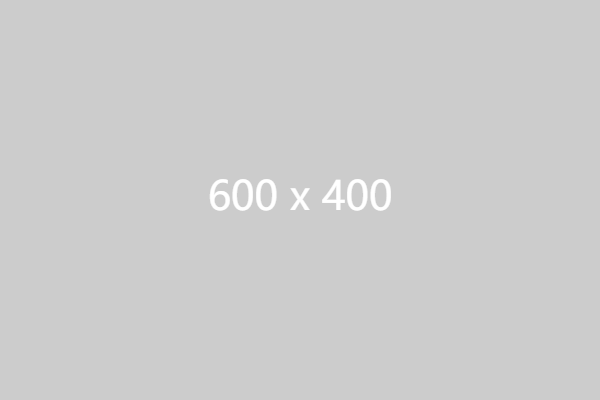
\includegraphics[width=0.8\textwidth]{example-image-2.png} %插入图片,[]中设置图片大小,{}中是图片文件名
    \caption{example\_caption} %最终文档中希望显示的图片标题
    \label{example_label} %用于文内引用的标签
\end{figure}

% 一行三张子图并排示意
\begin{figure}[htbp]
  \begin{subfigure}{0.31\textwidth}
    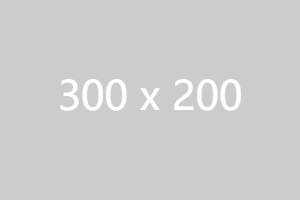
\includegraphics[width=\linewidth]{example-image-1.png}
    \caption{示意图1} \label{fig:9aaa}
  \end{subfigure}%
  \hspace*{\fill}   % maximize separation between subfigures
  \begin{subfigure}{0.31\textwidth}
    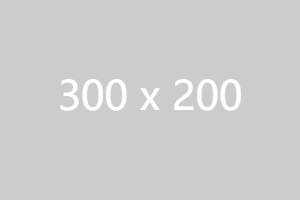
\includegraphics[width=\linewidth]{example-image-1.png}
    \caption{示意图2} \label{fig:9bbb}
  \end{subfigure}
  \hspace*{\fill}   % maximizeseparation between subfigures
  \begin{subfigure}{0.31\textwidth}
    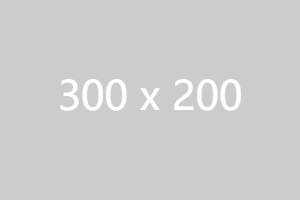
\includegraphics[width=\linewidth]{example-image-1.png}
    \caption{示意图3} \label{fig:9ccc}
    \end{subfigure}
\caption{一行三张子图并排示意}
\label{qmix-train}
\end{figure}


% 2*2四张子图示意
\begin{figure}[htbp]
  \begin{subfigure}{0.48\textwidth}
    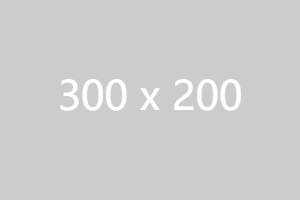
\includegraphics[width=\linewidth]{example-image-1.png}
    \caption{示意图1} \label{fig:8a}
  \end{subfigure}%
  \hspace*{\fill}   % maximize separation between subfigures
  \begin{subfigure}{0.48\textwidth}
    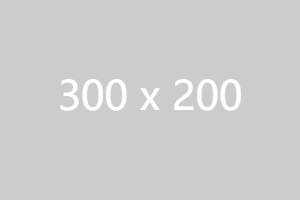
\includegraphics[width=\linewidth]{example-image-1.png}
    \caption{示意图2} \label{fig:8b}
  \end{subfigure}\\
  %\hspace*{\fill}   % maximizeseparation between subfigures
  \begin{subfigure}{0.48\textwidth}
    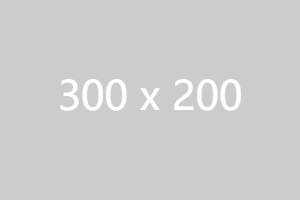
\includegraphics[width=\linewidth]{example-image-1.png}
    \caption{示意图3} \label{fig:8c}
  \end{subfigure}
  \hspace*{\fill}   % maximize separation between subfigures
  \begin{subfigure}{0.48\textwidth}
    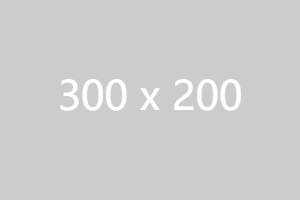
\includegraphics[width=\linewidth]{example-image-1.png}
    \caption{示意图4} \label{fig:8d}
  \end{subfigure}
\caption{2*2四张子图示意} \label{fig:8}
\end{figure}

%插入一个表格

\begin{table*}[t]
\centering
\caption{这是一个表注示例}
\begin{tabular}{|l||c|c|c|c|c|c|}
\hline
 {\textbf{攻击方法}}							&  黑/白盒攻击	&  定向/非定向 	& 特定/通用 	& 扰动范数 & 学习方式 		& 攻击强度  \\ \hline\hline
L-BFGS~ 		&  White box		&  Targeted					& Image specific			& $\ell_{\infty}$ 	& One shot		& $***$	\\ \hline
FGSM~		&  White box		&  Targeted					& Image specific			& $\ell_{\infty}$	& One shot		& $***$ \\ \hline
BIM \& ILCM~&  White box		& Non targeted				& Image specific			& $\ell_{\infty}$	& Iterative		& $**$$**$ 	\\ \hline
JSMA~		&  White box		& Targeted					& Image specific			& $\ell_{0}$	& Iterative			& $***$ 	\\ \hline
One-pixel~	& Black box		& Non Targeted		& Image specific		& $\ell_0$		& Iterative	& $**$ \\ \hline
C\&W attacks~ & White box	& Targeted	&	Image specific		&	$\ell_0, \ell_2, \ell_{\infty}$	&	Iterative & $*****$ \\ \hline
DeepFool~ & White box	& Non targeted		& Image specific		& $\ell_2, \ell_{\infty}$	& Iterative	& $**$$**$ \\ \hline
Uni. perturbations~ & White box	& Non targeted & Universal &	$\ell_2, \ell_{\infty}$ & Iterative & $*****$ \\ \hline
UPSET~ & Black box	& Targeted		& Universal 	&  $\ell_{\infty}$ & Iterative & $**$$**$ \\ \hline
ANGRI~ & Black box	& Targeted		& Image specific	& $\ell_{\infty}$ &	Iterative & $**$$**$ \\ \hline
Houdini~ & Black box		& Targeted		& Image specific	& $\ell_2, \ell_{\infty}$ & Iterative & $**$$**$ \\ \hline
ATNs~ & White box			& Targeted		& Image specific	& $\ell_{\infty}$ & Iterative & $**$$**$ \\ \hline
\end{tabular}
\end{table*}

%再插入另一种表格
\begin{table}[H]
\caption{我们的准确率真是太高啦}
\centering
\begin{tabular}{ccccc}
\hline  
\textbf{method} & \textbf{WR} & \textbf{FR} & \textbf{err} & \textbf{top} \\ 
\hline  
方法1 & 92.00\% & 2.00 & 19.07  & 5.66\\
方法2 & 99.00\%   & 9.76  & 18.94 & 7.83\\
方法3 & 96.00\%   & 1.01  & 24.09  & 9.08\\
方法4 & 99.99\%   & 4.66  & 40.69 & 4.21\\
\hline
\end{tabular} 
\end{table} 

\section{前景与展望}
本届赛制改革,合并科技、创业两类,可加入一些与商业相关的内容

\section{结论}
关于结论

\end{spacing}

\begingroup
\setstretch{2.0}    %行距2
\setlength{\bibsep}{0pt}    %段前段后0
\begin{adjustwidth}{0.42cm}{0.42cm} %左右缩进0.42cm
\bibliography{references}
\end{adjustwidth}
\endgroup

\end{document}
